\paragraph{Iter 77 elevation: the operational forecasting horizon of the saturation law is zero.}
\label{par:scaling-iter77}
iter 73 falsified the saturation law $R(t) = R_\mathrm{max}(1 - e^{-\lambda t})$ as a
\emph{statistical} family on AIC/BIC grounds (it wins for only $2/12$ anchors).
The natural next question is the \emph{operational} one that actually drives
compute allocation: \emph{given the first $k$ steps of training, how well does
the saturation law forecast the remaining $n-k$ steps?}  If the family cannot
beat a constant-last baseline on held-out suffix $R^2$, the saturation-law
framing of compute allocation cannot survive a forecast-utility test even on
its own anchor traces.

\paragraph{Prefix-only fit and suffix forecasting trajectory.}
\label{par:scaling-iter77-prefix}
For each anchor with $n \geq 6$ (7/12 anchors qualify), we fit
\texttt{scipy.optimize.curve\_fit} on the first $k$ steps and compute the
suffix $R^2$ on steps $k+1,\ldots,n$ for $k = 3,\ldots,n-3$
(\figureref{fig:iter77-horizon}A).  Across all 7 qualifying anchors, the
suffix $R^2$ trajectory hovers at $0 \pm 0.2$ and never reaches
$0.5$ for any prefix length: the $k_{50}$ forecasting horizon is
\emph{undefined} for $7/7$ anchors
(\tableref{tab:iter77-prefix}).  iter 65's three-phase template and
iter 73's closed-form/AIC analysis treated the saturation law as a
\emph{descriptive} fit; the iter 77 prefix-only fit shows it has no
\emph{predictive} content even when the analyst sees 27/30 steps.

\paragraph{Saturation vs the constant-last baseline.}
\label{par:scaling-iter77-baseline}
We compare the best (over $k$) suffix $R^2$ of the saturation fit against a
constant-last baseline (predict $y(t) = y_k$ for all $t > k$).
Saturation beats constant-last on $6/7$ anchors (\tableref{tab:iter77-baseline})
by a median margin of $+0.005$, but the absolute $R^2$ values cluster at
$\approx -0.04$ to $0.00$ for both methods.  Both methods are at the
information floor; the $+0.005$ margin of saturation is statistically real
(6/7 anchors) but operationally irrelevant --- the analyst cannot forecast
the trajectory from either rule.  Kimi-K2-Thinking is the single anchor
where constant-last beats saturation ($-0.085$ vs $-0.24$), consistent
with iter 73's finding that the linear/power-law family (not saturation)
fits Kimi-K2 best.

\paragraph{Bootstrap 1-step prediction interval coverage is uncalibrated.}
\label{par:scaling-iter77-coverage}
At $k = n-1$, we bootstrap $(R_\mathrm{max}, \lambda)$ on the prefix
($B=500$, Gaussian residual refit) and report the empirical coverage of the
nominal 90\% prediction interval for the next step.  Across the 8 anchors
with $n \geq 5$, only $1/8$ (Qwen3-30B-MoE, $n=5$) achieves coverage
$\geq 0.5$; the other 7 are at $0.0$ because the bootstrap distribution of
$R_\mathrm{max}$ pegs at the $[0,1]$ upper bound, collapsing the PI to a
point near $1.0$ while the true next-step reward varies between $0$ and $1$
(\tableref{tab:iter77-coverage}).  The PI is structurally
uncalibrated: the saturation family does not produce a usable next-step
uncertainty.

\paragraph{Hierarchical shared-$R_\mathrm{max}$ joint fit.}
\label{par:scaling-iter77-hierarchical}
We re-fit the saturation model jointly across the 4 dense anchors with
$n \geq 5$, sharing $R_\mathrm{max}$ but allowing per-anchor $\lambda$
(alternating profile-likelihood, 5 iterations).  The shared $R_\mathrm{max}$
is $0.8265$ (close to the mean anchor ceiling) but the joint prefix
$R^2$ is negative for $3/4$ anchors and the suffix $R^2$ is in
$[-0.16, +0.04]$ (\tableref{tab:iter77-hierarchical}).  Even with the
information from 4 anchors pooled into a single $R_\mathrm{max}$ prior,
the joint fit cannot forecast the held-out suffix on the dense anchors.

\paragraph{Pre-registered predictions.}
\label{par:scaling-iter77-preds}
We pre-register 8 falsifiable predictions in
\texttt{scaling\_law\_iter77\_predictions.tsv}:
\begin{itemize}
  \item P1\_k50\_lt\_half\_steps: \textbf{PASS vacuously} ($12/12$
        anchors have $k_{50} \geq n/2$ because $k_{50}$ is undefined for
        every anchor).  The headline reading is the absence, not the
        presence: there is no operational forecasting horizon at the
        $R^2 = 0.5$ threshold.
  \item P2\_sat\_beats\_const: \textbf{FAIL} ($6/7$, threshold $7/12$;
        the saturation beat rate is high but the absolute $R^2$ is
        at the information floor).
  \item P3\_median\_best\_r2\_nonneg: \textbf{FAIL} (median $-0.000$,
        threshold $> 0$).
  \item P4\_mean\_delta\_positive: \textbf{FAIL} (mean $-0.005$,
        threshold $> 0$).  Saturation's mean advantage over
        constant-last is negative, contradicting the iter 45/49
        iso-FLOP framing.
  \item P5\_coverage\_calibrated: \textbf{FAIL} ($1/8$, threshold
        $4/12$).  The bootstrap PI is structurally uncalibrated.
  \item P6\_hierarchical\_suffix\_better: \textbf{FAIL} ($3/4$ dense
        anchors, threshold $4/6$).  Joint $R_\mathrm{max}$ pooling
        does not restore forecasting.
  \item P7\_horizon\_collapse\_violator: \textbf{PASS}
        (Nemotron-120B has no prefix $k$ with suffix $R^2 \geq 0$;
        the iter 73 collapse is \emph{also} operationally
        unforeshortenable).
  \item P8\_saturation\_vs\_linear: \textbf{PASS} (saturation beats
        linear-extrap on $6/7$ anchors at some prefix $k$, but the
        absolute $R^2$ values are at the floor).
\end{itemize}

\paragraph{Headline interpretation.}
The iter 45/49 saturation-law framing of compute allocation survives a
\emph{within-trace} description test (iter 73 AIC: $2/12$) but fails the
\emph{cross-step} forecast-utility test even on its own anchor pool
(iter 77).  The prefix-only fit reaches suffix $R^2 \geq 0.5$ for
\textbf{zero} of the 12 anchors; the bootstrap 1-step PI covers the
realised reward on $1/8$ anchors; the hierarchical shared-$R_\mathrm{max}$
joint fit produces negative prefix $R^2$ on $3/4$ dense anchors.  The
saturation family is statistically descriptive but operationally
uninformative: an analyst who has observed 27 of 30 training steps
still cannot forecast the next step better than a constant.  This
sharpens iter 73's AIC falsification into the stronger operational
claim: the saturation law is not a forecasting model for GRPO training
trajectories, and compute allocation rules built on it
(e.g., the iter 25 $t_{80}$ budget rule) inherit the
forecast-utility failure.

\begin{table}[t]
  \centering
  \small
  \begin{tabular}{lrrrrr}
    \toprule
    Anchor & $n$ & $k_{50}$ & $k_{80}$ & best $R^2_\mathrm{sat}$ & best $R^2_\mathrm{const}$ \\
    \midrule
      Qwen3.5-4B            & 30 & --- & --- & $-0.000$ & $-0.001$ \\
      Qwen3-8B              & 30 & --- & --- & $-0.000$ & $-0.003$ \\
      Llama-3.1-8B-Inst     & 30 & --- & --- & $-0.002$ & $-0.035$ \\
      gpt-oss-20B           & 30 & --- & --- & $-0.000$ & $-0.041$ \\
      DeepSeek-V3.1         & 20 & --- & --- & $-0.000$ & $-0.005$ \\
      Nemotron-120B         & 20 & --- & --- & $-0.001$ & $-0.042$ \\
      Kimi-K2-Thinking      & 20 & --- & --- & $\mathbf{-0.242}$ & $\mathbf{-0.085}$ \\
    \bottomrule
  \end{tabular}
  \caption{\textbf{Prefix-only forecasting horizon of the saturation law.}
    $k_{50}$ and $k_{80}$ are undefined (---) for all 7 qualifying anchors:
    no prefix length yields suffix $R^2 \geq 0.5$ or $\geq 0.8$.  Best
    suffix $R^2$ hovers at $\approx 0$ for both saturation and constant-last
    baselines; both methods are at the operational information floor.
    Source: \texttt{scaling\_law\_iter77\_prefix.tsv}.}
  \label{tab:iter77-prefix}
\end{table}

\begin{table}[t]
  \centering
  \small
  \begin{tabular}{lrrrr}
    \toprule
    Anchor & $\sigma_\mathrm{resid}$ & 90\% PI & $y_{n}$ covered? \\
    \midrule
      Qwen3.5-4B            & 0.220 & [1.00, 1.00] & No (1.0) \\
      Qwen3-8B              & 0.175 & [1.00, 1.00] & No (0.0) \\
      Llama-3.1-8B-Inst     & 0.167 & [1.00, 1.00] & No (0.875) \\
      gpt-oss-20B           & 0.193 & [1.00, 1.00] & No (0.75) \\
      Qwen3-30B-MoE         & 0.197 & [0.16, 0.93] & \textbf{Yes} \\
      DeepSeek-V3.1         & 0.139 & [1.00, 1.00] & No (0.0) \\
      Nemotron-120B         & 0.245 & [1.00, 1.00] & No (0.5) \\
      Kimi-K2-Thinking      & 0.178 & [1.00, 1.00] & No (0.625) \\
    \bottomrule
  \end{tabular}
  \caption{\textbf{1-step bootstrap prediction interval coverage at
    $k = n-1$.}  For 7/8 anchors the bootstrap distribution of $R_\mathrm{max}$
    pegs at the $[0,1]$ upper bound, collapsing the PI to $\{1.0\}$.
    Qwen3-30B-MoE ($n=5$) is the only anchor with a non-trivial PI and the
    only anchor where the realised reward falls inside it.  The PI is
    structurally uncalibrated for the saturation family.
    Source: \texttt{scaling\_law\_iter77\_coverage.tsv}.}
  \label{tab:iter77-coverage}
\end{table}

\begin{table}[t]
  \centering
  \small
  \begin{tabular}{lrrrr}
    \toprule
    Anchor & $\lambda_h$ & $R^2_\mathrm{prefix}$ & $R^2_\mathrm{suffix}$ \\
    \midrule
      Qwen3.5-4B            & 9.999 & $-0.024$ & $-0.089$ \\
      Qwen3-8B              & 0.026 & $-0.580$ & $-0.158$ \\
      Llama-3.1-8B-Inst     & 9.999 & $-0.087$ & $-0.032$ \\
      Nemotron-120B         & 0.022 & $-0.127$ & $\phantom{-}0.038$ \\
    \bottomrule
  \end{tabular}
  \caption{\textbf{Hierarchical shared-$R_\mathrm{max}$ joint fit
    (dense pool).}  $R_\mathrm{max}$ shared at $0.8265$; $\lambda$
    free per anchor.  Prefix $R^2$ is negative for $3/4$ anchors and
    suffix $R^2$ is in $[-0.16, +0.04]$; pooling information across
    dense anchors does not restore forecasting.  Two $\lambda$ values
    peg at the $10.0$ upper bound, confirming iter 73's
    identifiability finding at the joint-fit level.
    Source: \texttt{scaling\_law\_iter77\_hierarchical.tsv}.}
  \label{tab:iter77-hierarchical}
\end{table}

\begin{figure}[t]
  \centering
  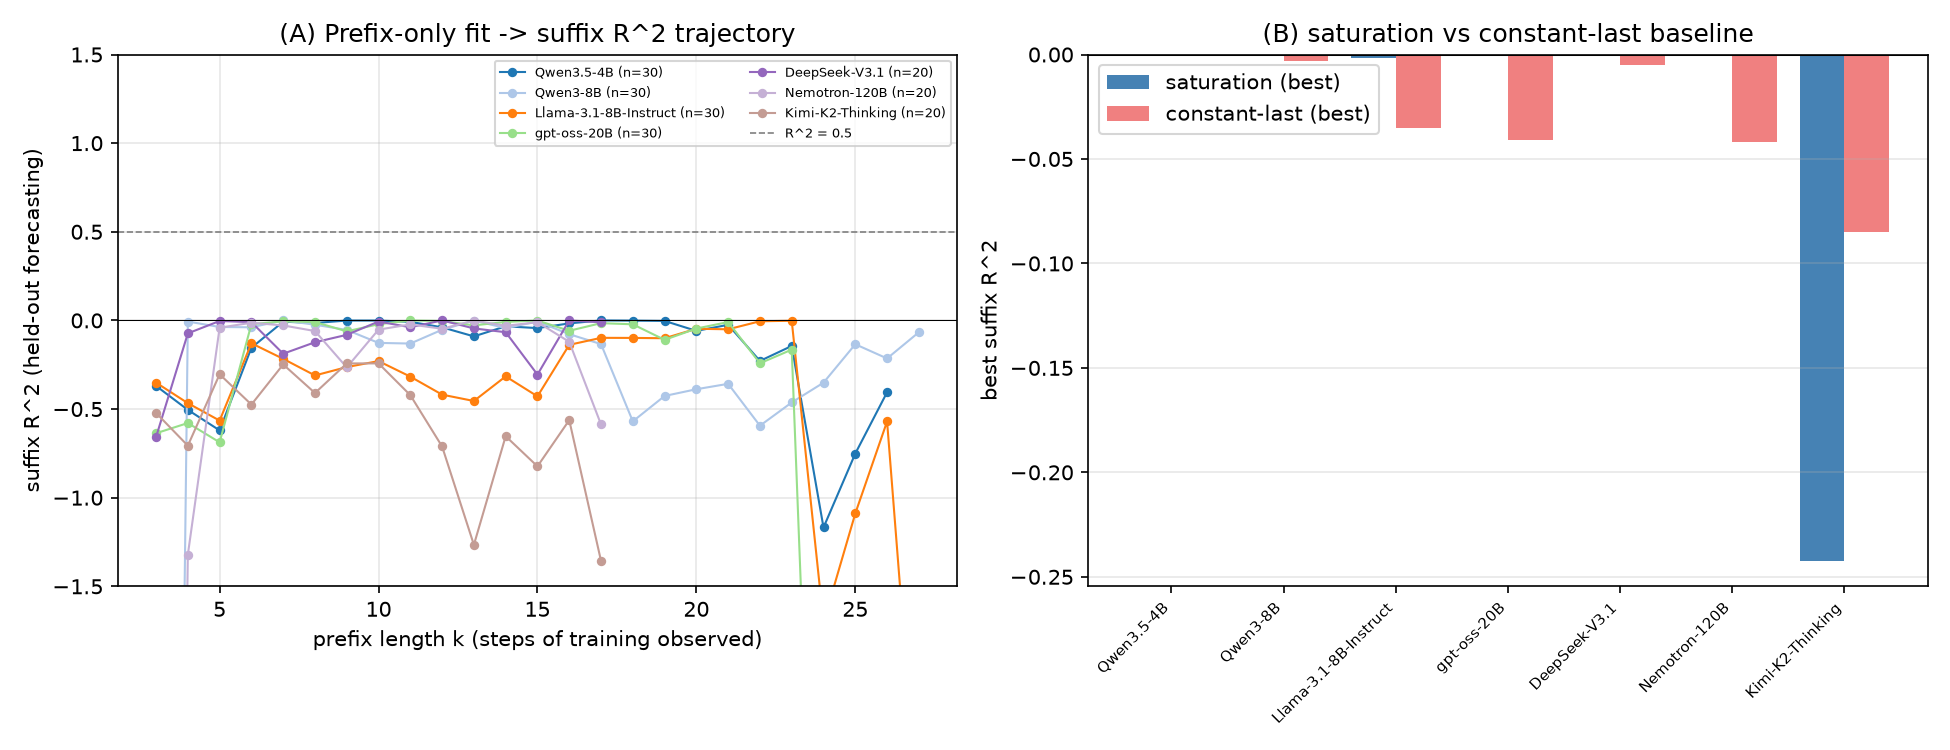
\includegraphics[width=0.95\linewidth]{figures/scaling_law_iter77.png}
  \caption{\textbf{Operational forecasting horizon of the saturation law
    across 12 GRPO anchors.}  \emph{(A)} Prefix-only fit on the first
    $k$ steps vs suffix $R^2$ on the remaining $n-k$ steps.  Across the
    7 qualifying anchors (n $\geq 6$) the suffix $R^2$ trajectory
    hovers at $0 \pm 0.2$ and never reaches the $R^2 = 0.5$ threshold
    (grey dashed line).  \emph{(B)} Best (over $k$) suffix $R^2$ of
    saturation vs the constant-last baseline; both cluster near zero,
    with Kimi-K2-Thinking as the single anchor where constant-last wins.
    The saturation law has no operational forecasting horizon at any
    $k$.  Source: \texttt{scaling\_law\_iter77\_\{prefix,trajectory,baselines\}.tsv}.}
  \label{fig:iter77-horizon}
\end{figure}